% !TEX root = ../main.tex
\section{Storm Kin} \label{sec::stormkin}

\DndDropCapLine{A}{sk anyone anywhere and they will give}
\textit{you a list of the things and people they lost to the ash storm.
That blasted cloud covered the entirety of the continent, leaving none unscarred.}

\hspace*{\fill} --- Iitus the scholar, "Of War and Thunder".

As the schism progressed, when the spire started spewing forth smoke and lava into the world, an immense ash storm gathered around the volcano, discharging lightning into anyone foolish enough to approach it.
As the years passed, the storm slowly subsided, leaving behind a strange race of being composed of ash, smoke, and lightning.
These being were named the zaloths, or storm kin, who adapted surprisingly well to the many kins of Yuadrem, and quickly found their new place in the world.

\subsection*{Ethereal Appearance}
The zaloths are tempests given physical shape, and their form reflects this.
They are composed of ash smoke, with strange forces shaping them into humanoid form.
Born from storm, they are in constant turmoil, and lightning sparks and cackles incessantly inside their bodies.

It is social norm for zaloths to clothe themselves in linen wrappings to cover their bodies, and it is not unusual for them to wear clothes or armor over these wrappings.
When they were formed, they also took the qualar of the unfortunate sentient creatures that were atop or near the spire, thus retaining their sentience.

Zaloths are not known to age or reproduce, and as such it's hard to tell if they'll be able to survive too long as a species.
They are thus extremely appreciative of their chance to experience life on Yuadrem, and are commonly known to be existentialists, looking to maximize their experiences in number and intensity.

When a zaloth suffers a mortal wound it does not die in a traditional sense, but the matter composing its body coalesces into a zaloth quintessent, a small cloud of ash.
This cloud does not retain its sentience, but it is somewhat able to keep its memories and experiences, and eventually merges into the atmosphere, becoming part of Yuadrem in a sense.

\subsection*{Distributed and Nomadic}
While a small group of zaloths established themselves in the city of Jan'krug at the top of the spire, the vast majority of the storm kin immediately started roaming the world alone or in small groups, looking for experiences.
Due to this, it is very rare to encounter an established zaloth community or zaloths living permanently in a city or town.
Nowadays, they are found wondering the land in caravans, circuses or as lone adventurers, eternally seeking new experiences.

When a wandering zaloth group meets another, it is common for them to celebrate this encounter by throwing a party in commemoration of their common heritage.
During this event, the members of the different groups conduct a ritual known to them as the mingling, where they allow their bodies to fuse, and thus share with each other their memories and experiences.

\subsection*{Presence in the World}
Due to their rarity, the other kins generally treat them with wonder and even admiration.
Many schools of thought regard the zaloths as sages due to the wisdom obtained in their nomadic ways, and their unique viewpoint on life and the world is appreciated by any who seek knowledge.

This however does not mean that all zaloths describe themselves as savant.
On the contrary, some of them give in to their inherent chaotic nature and become agents of turmoil, seeking paramount experiences via extreme means.
While their methods are frowned upon by more orthodox zaloths, they are far from being a pariah; they engage in mingling as commonly as any other zaloth.

\subsection*{Life of Adventure}
Due to the existentialist nature of the zaloths, a life of adventure is the most natural lifestyle that comes to them.
However, most zaloths are far from reckless, and while they can find dangers in their travels, they are careful to avoid mortal danger.
To the storm kin, any zaloth's death is a tragedy, and they prioritize the life of any of their kin over that of all other creatures.

A traveling zaloth will try all sorts of activities, independent of their nature and intensity.
Ever seeking new experiences, it is equally likely to encounter a zaloth engaging in quiet appreciation of nature, martial combat against formidable enemies, or joining in on other species' religious rituals.
Or even all of these activities on the same day.

\subsection*{Zaloth Names}
Due to the special conditions to their coming into the world, zaloths are born without names.
A zaloth usually chooses a name for itself after years, decades or even centuries of travel, and while it is nameless it is referred to using a feat or special characteristic that defines it.
The names that a zaloth chooses are commonly taken from other cultures or carefully designed by it.

\paragraph{Names} Basks-in-the-Sun, City-Swimmer, Dreams-of-Sleep, Dusk-Skin, Far-From-Water, Forest-Child, Has-no-Regrets, Head-in-Clouds, Iron-Fists, Mumbles-when-Speaks, Sees-All-Colors, Six-Coins, Somber-Mind, Sleeps-with-Open-eyes, Stands-in-Shallows, Swift-Legs, Takes-in-Light.

\begin{figure}[!t]
    \centering
    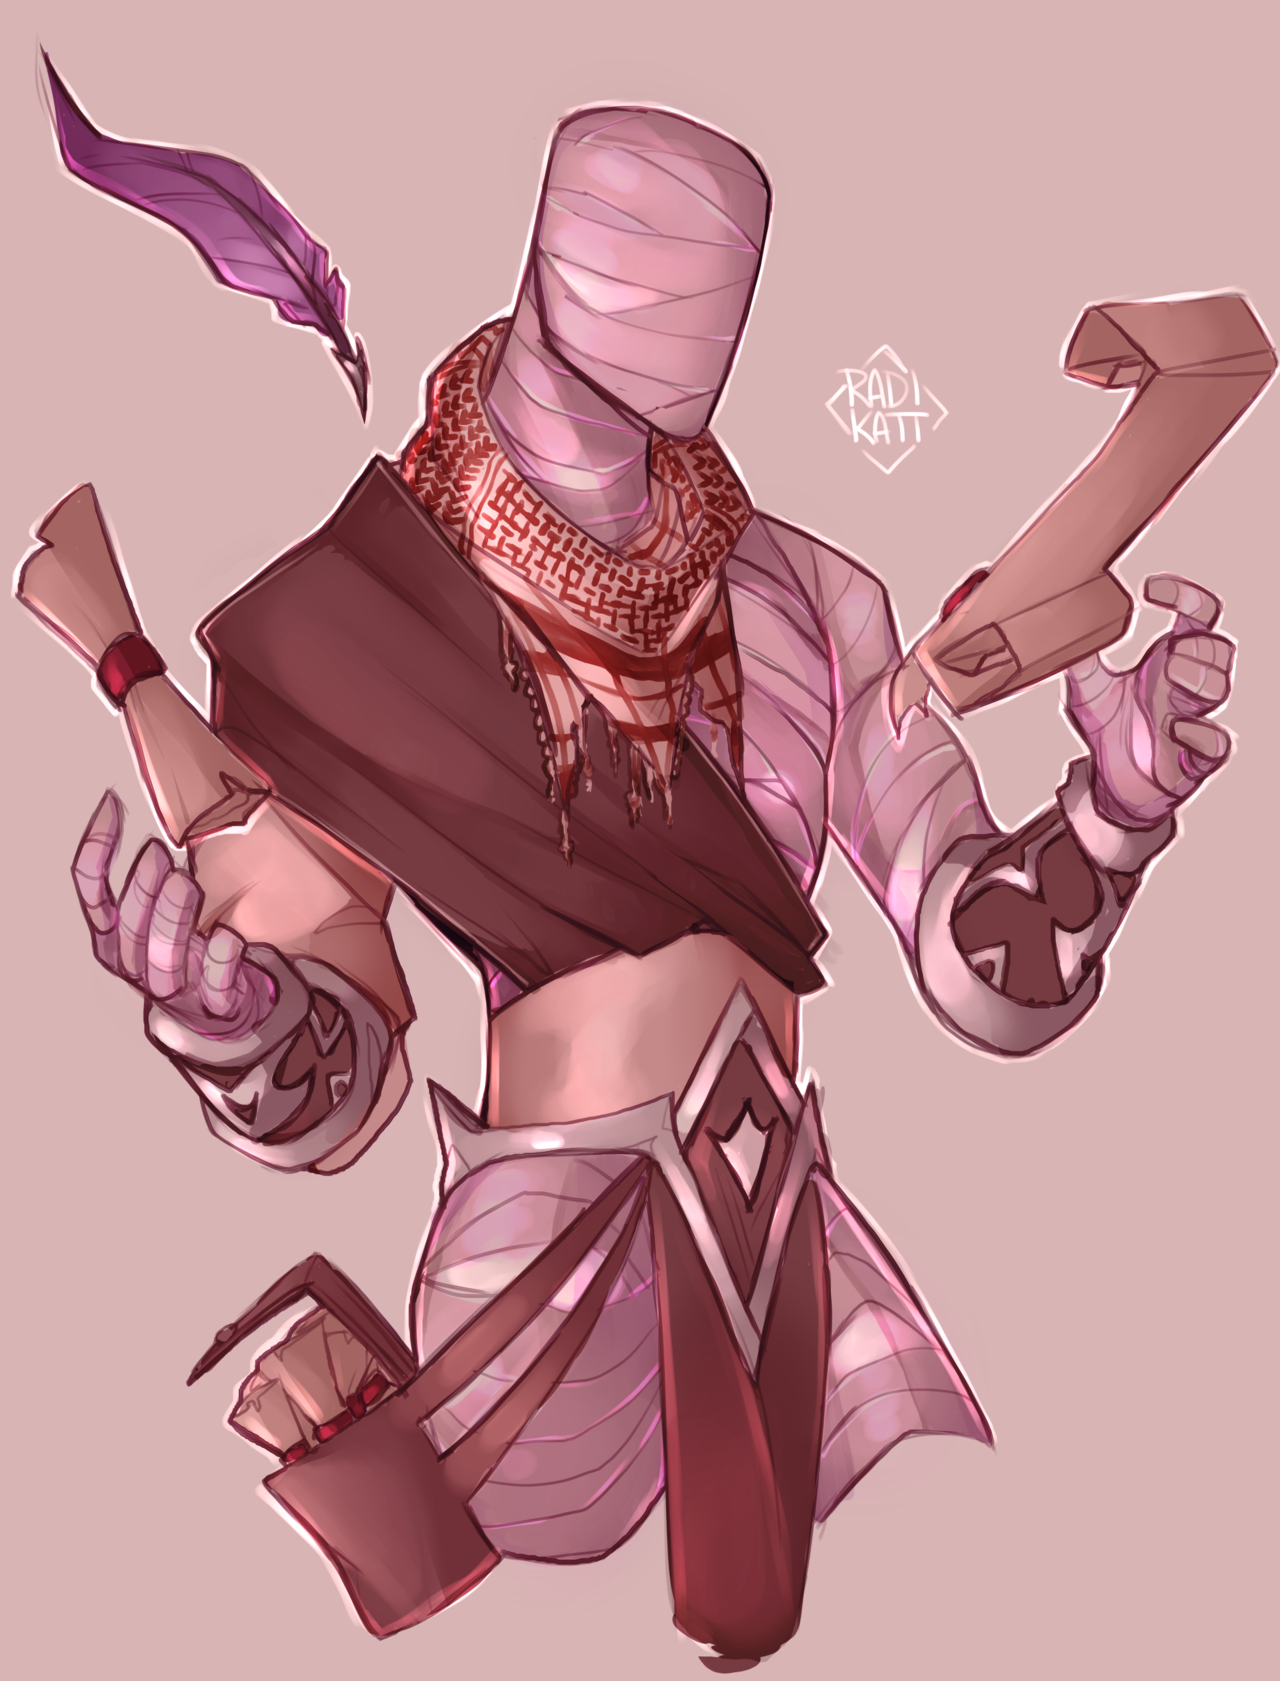
\includegraphics[width=0.48\textwidth]{04kins/img/20zaloth_scholar.png}
\end{figure}

\subsection*{Traits}
Your zaloth character has an assortment of traits related to its unique nature and nomadic lifestyle.

\subparagraph{Ability Score Increase} Your Charisma score increases by 1, and your Intelligence score increases by 1.

\subparagraph{Age} Born from an ash storm, a zaloth is thrust into adulthood, retaining some of the memories of the tall one from which it acquired its qualar as a blurry image.
Zaloths are not known to die from natural causes, and all of them are about 673 years old.

\subparagraph{Alignment} Most zaloth tend toward chaos, with little regard for the affairs of civilizations.
Due to their curious nature and lifestyle, zaloths move with the red tide.

\subparagraph{Size} Zaloths stand between 1.5 and 1.8 meters, and are practically weightless due to their unique composition.

\subparagraph{Speed} Your base walking speed is 9 meters.

\subparagraph{Dual Nature} You are both humanoid and elemental.
You can be affected by an effect if it works on either of these two creature types.

\subparagraph{Incorporeal} You are immune to poison damage, and cannot be affected by poison or disease.
Additionally, you don't need to eat or drink.

% \subparagraph{Hover} Instead of walking, your can choose to hover up to 1 feet over the ground.
% You can still be thrown into the ground if you are knocked prone, but you only need 5 feet of movement to stand up and don't provoke attacks of opportunity when you do so.

\subparagraph{Radiant} You give off dim light in a 3-meter radius and have disadvantage on Dexterity (Stealth) checks.
You cannot block this light with any clothing or armor.

\subparagraph{Telepathic} You can speak telepathically to any creature you can see within 9 meters of you.
Your telepathic utterances are in a language you know, and the creature understands you only if it knows that language.
Your communication doesn't give the creature the ability to respond to you telepathically.

\subparagraph{Silent Speaker} You can ignore the verbal components of spells.

\subparagraph{Languages} You can understand, read and write two languages of your choice, but you are unable to speak.
You can understand a very limited vocabulary of jantherlin, but your vocabulary consists of only individual words without context.

\subsubsection{Gale Zaloth}
Different zaloths have a stronger tendency towards different elements of the ash storm from which they were born.
Gale zaloths are attuned to the shifting, violent winds of the storm, and they reflect this with their erratic movements and shifting conversation subjects.
% A constant breeze can be felt around them, a grim reminder from the ash clouds.

\subparagraph{Ability Score Improvement} Your Dexterity score increases by 1.

\subparagraph{Stormbound} Wherever you go, you carry some of the storm with you.
A light breeze can be permanently felt in a 3-meter radius around you, moving in a random direction every turn.
The wind of this breeze displaces all smoke, gases, and very light objects inside its radius.
You can choose to end or restart this effect as a free action.

\subparagraph{Potent Quintessent} When you drop to 0 hit points, your desire to live manifests as a strong shockwave, sending any creature standing near you flying.
All creatures that stands in a 3-meter radius around you must succeed on a DC of 12 + your Constitution modifier Strength saving throw.
On a fail, a creature takes 1d6 force damage, is pushed 12 meters, and is knocked prone.
On success, a creature only takes half the damage, and isn't pushed or knocked prone.
You can use this ability once per short rest.

\subparagraph{Wind Given Form} You know the gust cantrip.
Once you gain your 3rd hit die, you can cast the feather fall spell.
Once you gain your 5th hit die, you can cast the dust devil spell as a 2nd level spell, requiring no material components.
Charisma is your spellcasting ability for these spells, and you can use each only once per short rest.

\subsubsection{Thunder Zaloth}
Thunder zaloths are attuned to the fleeting, fierce lightning.
They reflect this relation with their quick movements and sparking personalities.

\subparagraph{Ability Score Improvement} Your Charisma score increases by 1.

\subparagraph{Instant Step} You can expend your movement and a bonus action to transport instantly to a location up to your movement speed away that you can see.
Any creature standing in the straight line between the two positions must succeed on a DC 8 + your Constitution modifier Dexterity saving throw, taking 1d8 lightning damage on a failure.
You can do this a number of times equal to your Charisma modifier (Minimum of 1), and regain all expended uses when you complete a short rest.

\subparagraph{Elemental Resistance} You have resistance to lightning damage.

\subparagraph{Electricity Given Form} You know the shocking grasp cantrip.
Once you gain your 3rd hit die, you can cast the thunderwave spell as a 2nd level spell.
Once you gain your 5th hit die, you can cast the shatter spell as a 2nd level spell.
Charisma is your spellcasting ability for these spells, and you can use them only once per short rest.

\subsubsection{Ash Zaloth}
Ash zaloths are attuned to the destructive force of the spire, given form in the ash storm.
They embody the violence of the storm, and have affinity towards inflicting and receiving pain.

\subparagraph{Ability Score Improvement} Your Strength score increases by 1.

\subparagraph{Storm Conduit} The chaos of combat stirs your inner storm.
Once per round, you can deal an extra 1d4 fire damage to one creature you hit with an unarmed strike or an attack made with a metal weapon.
At 11th level, this damage increases to 2d4.
You can do this a number of times equal to your Charisma modifier (Minimum of 1), and you regain all expended uses when you complete a short rest.

\subparagraph{Elemental Resistance} You have resistance to fire damage.

\subparagraph{Flame Given Form} You know the produce flame cantrip.
Once you gain your 3rd hit die, you can cast the burning hands spell as a 2nd level spell.
Once you gain your 5th hit die, you can cast the Aganazzar's scorcher spell as a 2nd level spell.
Charisma is your spellcasting ability for these spells, and you can cast them once per short rest.

\subsubsection{Hail Zaloth}
Rarest of their species, the hail zaloths are the youngest of the zaloth, embodying the freezing hail into which the ash storm eventually decanted.
While still existentialist, they approach their curiosity in a calmer fashion, preferring the stillness of nature to the rowdiness of civilized society.

\subparagraph{Ability Score Improvement} You Wisdom score increases by 1.

\subparagraph{Cryogenic Stillness} You can choose to temporarily freeze your entire body, granting you extreme resilience.
As an action or reaction, you can instantly freeze, granting you immunity to slashing, piercing, and bludgeoning damage, apart from resistance to acid, force, lightning, necrotic, and thunder damage.
You also gain vulnerability to fire damage.
You are also affected by the slow spell for the duration of this trait without the possibility to roll saving throws.
You can maintain this effect for a number of turns equal to your Charisma modifier (minimum of 1), and must finish a short rest in order to use this trait again.

\subparagraph{Elemental Resistance} You have resistance to cold damage.

\subparagraph{Ice Given Form} You know the frostbite cantrip.
Once you gain your 3rd hit die, you can cast the ice knife spell as a 2nd level spell.
Once you gain your 5th hit die, you can cast the icy surface spell as a 2nd level spell.
Charisma is your spellcasting ability for these spells, and you can use them only once per short rest.

\begin{figure}[!b]
    \centering
    
\includegraphics[width=0.48\textwidth]{04kins/img/20zaloth_thunder.jpg}
\end{figure}



\newpage
